
\section{Setting up edge environments}
Unikernels, similar to traditional OSes can be booted directly from BIOS to hardware. Nevertheless, this is not flexible enough for cloud computing standarts, so hypervisors are used for on demand provisioning of unikernels. An example project is called Jitsu\cite{jitsu}, Just in time sumoning of unikernels. In that project, for every DNS request they are starting a unikernel to respond to that request. The working principle can be seen in \ref{fig:jitsu}.

\begin{figure}[htpb]
    \centering
    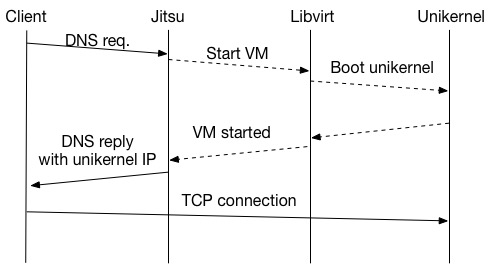
\includegraphics[width=0.8\textwidth]{figures/jitsu.jpg}
    \caption{Jitsu \cite{jitsu}} \label{fig:jitsu}
  \end{figure}

This scenario can also be achieved in Kubernetes. In kubernetes, incoming requests to the cluster are controlled with an API object called \textit{ingress}, and a custom DNS service with different rules can start up a unikernel (or any other process) to respond to the request. Jitsu project uses Xen and libvirt to manage their hypervisor.

This thesis was tested on Xen hypervisor and a unikernel specific execution environment called Solo5 \cite{solo5}. Used IoT device is Raspberry Pi and because it's currently not officially supported to install hypervisors on Raspberry Pi's, unikernels compiled for unix were used instead. This case also shows that, with this implementation it's actually possible to run any arbitrary binary on raspberry pi without any further modification.

\subsection{Type-2 Hypervisor}
It's possible to run unikernels on type-2 hypervisors, like virtualbox. This thesis did not aim to run them on type-2 hypervisors but there are project that do that , so it's possible by updating the provider methods, thus it's worthy to be mentioned for future work.

% todo:
\subsection{Type-1 Hypervisor}
The unikernel technology used by this project, MirageOS, is being developed by ex XEN developers. Naturally it has official support for Xen and all their examples can be compiled to Xen. 
\subsection{IoT Devices}

Raspberry Pi 3 has 1GB, 900 Mhz RAM and 4*ARM Cortex-A53,1.2 GHz CPU. Because it uses ARM, x64 hypervisors can not be ported easily. There is also no motivation for it, since Raspberry Pi's are not powerful machines and virtualisation is a resource hungry process. Nevertheless, there are projects for lightweight virtualization on Raspberry Pi.

